\documentclass[main.tex]{subfiles}

\begin{document}

% \chapter{Технічне завдання для дипломного проекту}
% \section{Найменування і область застосування}
% \section{Підстави для розробки}
% \section{Мета і призначення розробки}
% \section{Джерела розробки}
% \section{Технічні вимоги}
% \subsection{Вимоги до розроблюваного продукту}
% \subsection{Вимоги до програмного забезпечення}
% \section{Етапи розробки}

\newpart{part3}{ІАЛЦ.467100.003.ПЗ}
\tableofcontents

% I'm not yet sure, I need a translation, so that may change in the
% future
\newcommand\engacro[3]{\acro{#1}{\acroextra{(}#2\acroextra{) #3}}}

\specialchapter{Список скорочень}
\begin{acronym}[TCP/IPA]

  % To decrease spacing
  % \setlength\parskip{0ex}

  \engacro{AST}{Abstract Syntax Tree}{Абстрактне Синтаксичне Дерево}
  \acro{CAN}{Controller Area Network}
  \acro{CPU}{Central Processing Unit}
  \acro{DOSFS}{FAT-based file system}
  \engacro{DSL}{Domain-Specific Language}{Предметно-Орієнтована Мова}
  \engacro{EDSL}{Embedded Domain-Specific Language}{Вбудована Предметно-Орієнтована Мова}
  \acro{ELF}{Executable and Linkable Format}
  \acro{FPU}{Floating Point Unit}
  \acro{HRFS}{High Reliability File System}
  \engacro{IoT}{Internet of Things}{Інтернет Речей}
  \engacro{LTO}{Link Time Optimization}{Оптимізація Часу Зв'язування}
  \acro{MMU}{Memory Management Unit}
  \acro{NFS}{Network File System}
  \engacro{RAM}{Random Access Memory}{Оперативна Пам'ять}
  \acro{ROM}{Read-Only Memory}
  \engacro{RTOS}{Real-Time Operating System}{Операційна Система Реального Часу}
  \acro{SLOB}{Simple List of Blocks}
  \acro{SoC}{System on Chip}
  \acro{TCP/IP}{Transport Control Protocol/Internet Protocol}
  \acro{USB}{Universal Serial Bus}
  \acrodefplural{КПК}[КПК]{Карманні Портативні Комп'ютери}
  \acro{КПК}{Карманний Портативний Комп'ютер}
\end{acronym}

\specialchapter{Вступ}

У наші дні активно відбувається мініатюрізація пристроїв, швидкими темпами розвивається \ac{IoT}. Гігантськими кроками збільшується кількість пристроїв, що підключені до Інтернету. Експерти оцінюють, що до 2020-го року буде існувати до 50 мільярдів підключених пристроїв\cite{dave-evans:IoT}.

Це означає, що складність програмного забезпечення для вбудованих пристроїв буде зростати, оскільки їм тепер необхідно взаємодіяти з іншими пристроями за допомогою Інтернету, водночас зберігаючи довгу тривалість роботи і надзвичайно низькі вимоги до ресурсів.

Таким чином, вбудовані пристрої вимагають систем управління, що будуть полегшувати організацію складної роботи, зменшувати кількість помилок програміста, і водночас мати мінімальні вимоги до ресурсів процесора і оперативної пам'яті, бути легко переносимими на інші платформи і архітектури.

У рамках даного дипломного проекту ставиться завдання розробити систему управління для пристроїв з мінімальним обсягом пам'яті. Розробка буде вестися за допомогою мікроконтроллера STM32F407VGT6, що має має 192 Кб оперативної пам'яті. Однак, система має використовувати мінімум оперативної пам'яті і бути легко портованою на значно менш потужні мікроконтролери. Додатковою метою ставить оцінка сучасних інструментів, зокрема мов програмування, у рамках створення програмного забезпечення для вбудованих пристроїв.

При створенні програмного продукту було пройдено повний цикл його написання -- від постановки завдання, написання технічного завдання і вимог до продукту, до написання програмного забезпечення та тестування.

\chapter{Операційні системи для вбудованих пристроїв}
\section{Загальні положення}

Вбудована система це комп'ютерна система зі спеціалізованою функцією, що є частиною більшої механічної або електронної системи, і часто має обмеження реального часу. Система є вбудованою як частина цілого пристрою, що часто включає у себе апаратні засоби і механічні частини. Вбудовані системи контролюють велику кількість пристроїв, що є розповсюдженими. 99\% всіх вироблених мікропроцесорів використовуються як компоненти вбудованих систем\cite{embedded:99}.

Зазвичай, вбудовані комп'ютери, на відміну від комп'ютерів загального призначення, мають низькі витрати енергії, малий розмір, більший робочий діапазон і значно меншу ціну за одиницю. За це доводиться платити обмеженими процесорними ресурсами, що робить такі комп'ютери значно важчими для програмування і взаємодії. Сучасні вбудовані системи зазвичай базуються на мікроконтроллерах (центральні процесори, що мають інтегровану оперативну пам'ять і периферійні інтерфейси).

Оскільки вбудовані системи є спеціалізованими, інженери-конструктори можуть оптимізувати їх для зменшення розміру і ціни продукту, підвищення надійності і продуктивності. Деякі вбудовані системи випускаються серійно.

Вбудовані системи різняться від портативних пристроїв як цифрові годинникі і MP3 плеєри, до великих стаціонарних установок, як то світлофори, заводські контроллери, і великих комплексних систем як гібридні транспортні засоби, МРТ і авіаційна електроніка. Складність системи змінюється від простої, з одним мікроконтроллером, до дуже високої з кількома одиницями, периферією і мережею змонтованою всередині великого корпусу.

Із ростом складності системи, вони все більше потребують операційної системи, що може її зменшити для програміста.

Операційна система це системне програмне забезпечення, що управляє апаратними і програмними ресурсами, і надає обслуговує комп'ютерні програми. Операційна система виступає посередником між програмними додатками і апаратними функціями, як то ввід, вивід і алокація пам'яті, хоч код додатка зазвичай виконується апаратними ресурсами напряму. Операційні системи можна знайти в багатьох пристроях -- від ігрових консолей і мобільних телефонів до веб серверів і суперкомп'ютерів.

Прикладами популярних операційних систем для настольних комп'ютерів є Apple OS X, Linux і його варіанти, а також Microsoft Windows. Так звані мобільні операційні системи включають Android і iOS. Однак, існує набагато більше класів операційних систем, до яких входять вбудовані операційні системи і операційні системи реального часу.

Вбудовані операційні системи призначені для вбудованих комп'ютерних систем. Вони розробляються для роботи на малих машинах, таких як \acp{КПК}, і можуть працювати при обмежених ресурсах. Вони є компактними і надзвичайно ефективними.

Операційні системи реального часу це операційні системи, що гарантують обробку подій або даних за визначений короткий проміжок часу. Вони можуть бути одно- або багатозадачнимию. Якщо використовується багатозадачність, то використовуються спеціалізовані алгоритми планування для того, щоб гарантувати детермінізм. Подієві (event driven) системи переключаються між задачами на основі їх пріоритетів, коли системи з поділом часу переключаються на основі переривань годинника.

Одними із найбільш важливих частин операційної системи в контексті вбудованих систем є алокатор пам'яті і планувальник задач.

Алокатор пам'яті це частина системи відповідальна за алокацію і управління пам'яттю. Головною вимогою до управління пам'яті є надання можливості динамічно виділяти ділянки оперативної пам'яті програмам за запитом, звільнення і повторне використання цих ділянок після того, як вони більше не потрібні.

Планувальник задач це частина операційної системи, що визначає, яка задача має виконуватися в кожен момент часу. Зазвичай, він має можливість зупиняти активні задачі і починати нові.

\section{Огляд існуючих рішень}\label{existing-solutions}
Існує багато вбудованих операційних систем і часто вони перетинаються з операційними системами реального часу і надають можливості обох типів систем. Далі розглдаються найбільш популярні вбудовані операційні системи насьогодні.

\subsection{Embedded Linux}

Ядро Linux\cite{linux} пропонує широкий набір функціоналу, серед якого можна знайти безліч драйверів, підтримка великої кількості файлових систем, широкий вибір планувальників і алокаторів пам'яті. Однак, для зниження системних вимог, доводиться відмовлятися від більшості функцій, що надає ядро Лінукс.

Ядро Linux було портовано на велику кількість архітектур, в число яких входять такі як ARM, AVR32, MIPS, Xtensa. Ці архітектури використовуються у вбудованих системах. Однак Linux висуває досить високі вимоги до ресурсів системи. Мінімальний обсяг оперативної пам'яті, що вимагає система, дорівнює 4 мегабайтам, також Лінукс вимагає наявності \ac{MMU}, що перешкоджає його використанню в системах на нижній границі потужностей.

Незважаючи на це, Том Занусі модифікував ядро Лінукс і портував його на Intel Galileo\cite{linux-galileo}. Ця плата базована на мікроконтроллері Intel Quark SoC X1000, що має архітектуру Pentium і 1.6 мегабайт вбудованої оперативної пам'яті\cite{intel-galileo}.

Ядро розповсюджується під вільною ліцензією GPLv2.

\newcommand{\FIFO}[0]{SCHED\_FIFO}
\newcommand{\RR}[0]{SCHED\_RR}

Linux пропонує два планувальники реального часу\cite{linux:schedulers}: SCHED\_FIFO і SCHED\_RR. Основним режимом для реального часу є SCHED\_FIFO, що реалізує алгоритм планування first-in, first-out. Коли \FIFO{} задача починає своє виконання, вона продовжує своє виконання, поки добровільно не віддасть процесор, заблокується, або буде витіснена задачею з більшим пріоритетом. Задача не має квантів часу. Всі задачі з меншим пріоритетом не будуть виконуватися, доки задача з більшим пріоритетом не поступиться процесором. Дві задачі з однаковим пріорітетом не витісняють одна одну.

\RR{} схожий до \FIFO{}, за виключенням, що задачам надаються кванти часу на базі їх пріоритету і задачі працюють, доки не вичерпають свій квант. Задачі не реального часу використовують стратагію SCHED\_NORMAL.

\subsection{VxWorks}

VxWorks\cite{vxworks} це операційна система реального часу зозроблена як власницьке програмне забезпечення Wind River. VxWorks призначена для вбудованих систем реального часу, що вимагають детермінованої продуктивності, і часто, проходження сертифікації безпеки і захищенності.

VxWorks підтримує архітектури Intel x86, MIPS, PowerPC, Freescale ColdFire, Intel i960, SPARC, Fujitsu FR-V, SH-4, ARM, StrongARM і xScale, і може працювати y режимах симетричної, асиметричної і змішаної багатопроцесорної обробки. Операційна система включає у себе багатозадачне ядро з витісняючим планувальником, засоби міжпроцесорної взаємодії і синхронізації, стек протоколів Bluetooth, \acs{TCP/IP}, \acs{USB}, \acs{CAN}, а також файлові системи \ac{HRFS}, \acs{DOSFS}, \ac{NFS}.

Мінімальний обсяг оперативної пам'яті дорівнює 20-ти кілобайтам.

VxWorks активно використовується в аерокосміній, захисній, автомобільній і робототехнічній галузях. Відомими прикладами використання є марсоходи Sojourner, Spirit, Opportunity\cite{vxworks:rovers}, загальна система ядра Boeing 787 Dreamliner\cite{vxworks:boeing}.

\subsection{FreeRTOS}

Насьогодні, FreeRTOS\cite{freertos} є найпопулярнішою операційною системою реального часу для вбудованих систем\cite{freertos:popular}. Її було портовано на 35 мікроконтроллерів, що мають наступні архітектури: ARM, AVR, HCS12, MicroBlaze, Cortus, MSP430, PIC, Renesas~ H8/S, SuperH, RX, x86, 8052, Coldfire, V850, 78K0R, Fujitsu MB91460, Nios~ II, TMS570, RM4x.

\begin{figure}[h]
  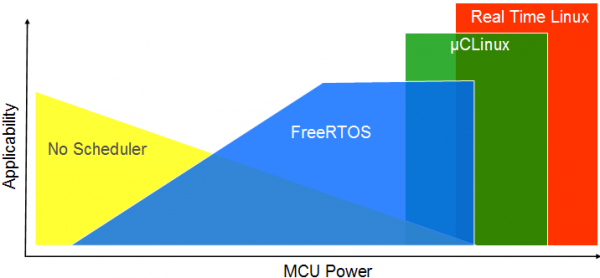
\includegraphics[width=\textwidth]{freertos-market-position}
  \caption{Положення FreeRTOS на ринку вбудованих операційних систем}
\end{figure}

Це дуже проста операційна система, що складається з чотирьох файлів на мові C. FreeRTOS надає методи для роботи з потоками, м'ютексами і семафорами, таймерами і чергами. Підтримується так званий tickless режим роботи (у цьому режимі переривання таймера відбуваються при нерівних інтервалах, і лише в міру необхідності).

Доступні чотири алокатори пам'яті:
\begin{itemize}
  \item Виділення пам'яті без можливості її звільнення.
  \item Простий алгоритм виділення і звільнення пам'яті без об'єднання вільних ділянок.
  \item Більш складний і швидкий алгоритм виділення і звільнення пам'яті з об'єднанням вільних ділянок.
  \item Обгортки навколо стандартної бібліотеки, що забезпечують взаємне виключення.
\end{itemize}

FreeRTOS має надзвичайно низькі вимоги до оперативної пам'яті. Планувальник вимагає 236 байт оперативної пам'яті, плюс 76 байти для кожної черги і 64 байти для кожної задачі.

Ядро розповсюджується під модифікованою вільною ліцензією GPLv2\cite{freertos:license}. Модифікація дозволяє залишати закритим код додатків, що використовують FreeRTOS і розповсюджуються у вигляді виконуваного коду, а також забороняє використання FreeRTOS у еталонних теста. Також доступна комерційна підтримка і ліцензія під ім'ям OpenRTOS\cite{openrtos}.

FreeRTOS має лише один планувальник задач -- Round Robin. Алгоритм ідентичний до того, що використовується в Linux. Задача з максимальним пріоритетом отримує процесор. Якщо існує кілька задач з однаковим пріоритетом, він виконує їх по черзі. Задачі з нижчим пріоритетом мусять очікувати.

Дуже важливо, щоб задачі за максимальним пріоритетом не займали 100\% процесорного часу, адже задачі з нижчим пріоритетом будуть заблоковані і ніколи не отримають процесорний час. Це фундаментальна проблема програмування систем реального часу.

\subsection{QNX Neutrino}

QNX\cite{qnx} це комерційна Unix-подібна операційна система спрямована в першу чергу на вбудовані системи. Операційна система має мікроядерну архітектуру. QNX Neutrino була портована на велику кількість платформ і працює на Intel 8088, x86, MIPS, PowerPC, SH-4, ARM, StrongARM, XScale.

Ядро QNX містить лише планувальник задач, міжпроцесну взаємодію, перенаправлення переривань і таймери. Все інше виконується як процеси рівня користувача, включаючи керування пам'яттю.

QNX має закриту ліцензію, але також має окрему ліцензію для академічного і некомерційного використання\cite{qnx:noncommercial}.

\chapterconslusions{}

У даному розділі було надано означення та основні ознаки вбудованих систем, а також було описано поняття та класифікація операційних систем і їх основних компонентів.

Насьогодні, вбудовані системи оточують людину усюди, а кількість таких систем із часом буде лише збільшуватися за рахунок розвинення ринку \acs{IoT}. Продовжується мініатюрізація комп'ютерів з одночасним розширенням їх обов'язків.

Саме тому важливо реалізувати ефективну операційну систему, що знизить навантаження на програміста і дозволить йому реалізувати швидке і надійне програмне забезпечення.

Існує багато операційних систем для вбудованих пристроїв. Багато із них надають можливості реального часу. Однією із найменших таких систем насьогодні є FreeRTOS, що надає лише базові можливості: алокатор пам'яті, планувальник задач і кілька примітивів синхронізації.

\chapter{Аналіз і вибір мови програмування}\label{chap:languages}

%\newcommand\LangC{Сі}
\newcommand\LangC{C}

\section{Загальні вимоги}

Програмування мікроконтролерів висуває певні вимоги до мови.

По-перше, мова має бути компілюєма, оскільки на дешевих мікроконтролерах дуже мало ресурсів для інтерпретації мови, або її компіляції. На більших платформах, інтерпретація можлива, але однаково вимагає додаткових витрат процесорного часу і пам'яті. Оскільки дана робота розглядає реалізацю операційної системи, що буде вимагати мінімального обсягу пам'яті, інтерпретація мови на мікроконтроллері неможлива.

По-друге, мова не повинна вимагати збирача сміття, або будь-якого іншої бібліотеки середовища виконання. Як і з інтерпретацією, це вимагає додаткових ресурсів, якими мікроконтролер часто не володіє.

По-третє, низькорівневе програмування схильне до програмних помилок, що важко знайти і виправити. На відміну від прикладного програмування, помилки на системному рівні частіше призводять до краху усієї системи. До найчастіших помилок можна віднести помилки виходу за границі буферу, помилки при роботі з динамічною пам'яттю, витік ресурсів, помилки синхронізації, виклик заборонених у певному контексті функцій. Це означає, що мови системного програмування мають приділяти особливу увагу питанню безпеки.

Також, для програмування операційних систем дуже важлива можливість контролювати розмітку пам'яті і робота з пам'яттю напряму. Додатковими плюсами є можливість вбудови асемблерних інструкцій, взаємодія з іншими мовами (зокрема мовою асемблера і \LangC{}), наявність якісного компілятора, що генерує швидкий код.

\section{C}

Мову \LangC{} було розроблено у 1972 році Денісом Рітчі у Bell Telephone Labaratories з метою написання операційної системи UNIX\cite{stewart-bill:history-of-c}. \LangC{} є однією із найпопулярніших у світі мов програмування за кількістю вже написаного програмного забезпечення, а також кількості програмістів.

Найпростіша програма мовою \LangC{} зображена на рисунку \ref{example:c}.

\begin{figure}[h]
  \centering
  \begin{BVerbatim}
#include <stdio.h>

// This is an example of comment
int main(void)
{
  printf("Hello, world!\n");

  return 0;
}
  \end{BVerbatim}
  \caption{Приклад найпростішої програми мовою \LangC{}}\label{example:c}
\end{figure}

Мова \LangC{} надає можливості прямого доступу до пам'яті, майже повний контроль над пам'яттю і потоком виконання, не має збирача сміття, або будь-якої бібліотеки середовища виконання. Також, \LangC{} має просту домовленість про виклики, що дозволяє легко використовуваи функції, написані на \LangC{}, майже з будь-якої іншої мови програмування, включаючи мову асемблера. Існують дуже потужні і стабільні компілятори, що генерують високоефективний машиний код. Все це робить \LangC{} гарним кандидатом.

Мова \LangC{} є \emph{де-факто} стандартом для написання вбудованих систем. Це перевірений роками інструмент, що довів свою ефективність і показав себе найкращим у класі вбудованих систем.

Однак, \LangC{} не можна назвати сучасною мовою. Її було розроблено майже 50 років тому і сьогодні не ведеться активних розробок з покращення і розвинення мови. Останній стандарт (C11) було випущено у 2011 році, але він вносить лише незначні покращення і не виправляє багатьох фундаментальних проблем мови \LangC{}.

Однією із серйозних проблем \LangC{} є типізація. Мова \LangC{} має слабку статичну типізацію; це означає, що всі типи перевіряються на етапі компіляції, але існують неявні приведення типу, що досить часто призводить до програмних помилок. Також, система типів є дуже примітивною, і не має корисних функцій, що характерні більш сучасним системам типів.

\section{Idris}\label{sec:idris}

Мова Idris\cite{idris} є чисто-функціональною мовою програмування з потужною системою типів, що підтримує залежні типи. Розробка мови ведеться з 2009 року\cite{idris:first-release}, тож мова є дуже молодою.

Код найпростішої програми мовою Idris наведено на рисунку \ref{example:idris}.

\begin{figure}[h]
  \centering
  \begin{BVerbatim}
module Main

main : IO ()
main = putStrLn "Hello, world!"
  \end{BVerbatim}
  \caption{Приклад найпростішої програми мовою Idris}\label{example:idris}
\end{figure}

Насьогодні, залежні типи не є широко-використовуваною технологією у програмуванні і використовуються здебільшого у науковому середовищі, а також ентузіастами мов програмування. Залежні типи стирають межу між типами і значеннями; типи стають звичайними значеннями, що дозволяє виконувати операції над типами, передавати їх як аргументи функцій і повертати їх із функцій. Тож можна мати різний тип в залежності від результатів обчислення певного значення, або іншого типу.

За допомогою залежних типів в Idris було побудовано систему ефектів. Система ефектів дозволяє розділити використання певних дій від їх конкретної реалізації. Наприклад, функція може використовувати функції логування, однак вибір їх конкретної реалізації залишається на функції, що врешті решт викличе виконання ефекту. Це можна назвати формою впровадження залежностей (dependency injection). 

\begin{figure}%[h]
  \centering
  \begin{BVerbatim}
module Effect.File

import Effects
import Control.IOExcept

FILE_IO : Type -> EFFECT

data OpenFile : Mode -> Type

open : (fname : String)
       -> (m : Mode)
       -> Eff Bool [FILE_IO ()]
                   (\res => [FILE_IO
                     (case res of
                       True => OpenFile m
                       False => ())])
close : Eff () [FILE_IO (OpenFile m)] [FILE_IO ()]

readLine  : Eff String [FILE_IO (OpenFile Read)]
writeLine : String -> Eff () [FILE_IO (OpenFile Write)]
eof       : Eff Bool [FILE_IO (OpenFile Read)]

Handler FileIO IO where { ... }
  \end{BVerbatim}
  \caption{Приклад використання залежних типів}\label{idris:dependent-types}
\end{figure}

Система ефектів також дозволяє керувати і розмежовувати доступ повних функції до певних ефектів. Наприклад, можна створити ефект для роботи з мережею; тоді можна обмежувати доступ до мережевих операцій на рівні окремих функцій -- компілятор може гарантувати під час компіляції, що певна функція не буде використовувати функції роботи з мережею.

Система ефектів і залежні типи можуть підвищити рівень надійності операційних систем, якщо правильно їх використовувати. За допомогою створення окремого класу блокуючих операцій, можна позбавитися від цілого класу проблем, що виникають при виклику блокуючих операцій з обробнику переривань. За допомогою ще інакшого ефекту, можна гарантувати вивільнення ресурсів, як то пам'ять або відкриті файлові дескриптори. За допомогою залежних типів можна накладати обмеження на виділення оперативної пам'яті, або навіть на кількість тактів процесора для певних функцій. В цілому, залежні типи це дуже потужних механізм для забезпечення перевірки певних припущень у самомоу коді програми і математичного доведення правильності програми.

Нажаль, Idris вимагає збирача сміття і великої бібліотеки часу виконання, що унеможливлює використання Idris напряму для створення програмного забезпечення для систем з обмеженою пам'яттю. Але можливо створити EDSL (embedded domain-specific language, вбудована предметно-орієнтована мова) на базі Idris для генерація коду для вбудованих систем і таким чином позбутися даних обмежень мови. Схожим чином було реалізовано мови Atom\cite{haskell:atom} і Ivory\cite{haskell:ivory}, але на базі мови Haskell\cite{haskell}.

\section{Nim}

\begin{figure}[!bp]
  \centering
  \begin{BVerbatim}
# This is comment

# All top-level statements are
# executed when program starts
echo "Hello, world!"
  \end{BVerbatim}
  \caption{Приклад найпростішої програми мовою Nim}\label{example:nim}
\end{figure}

Мова Nim\cite{nim} (раніше Nimrod) вперше зв'явилася у 2008 році. Це багатопарадигмена мова, що компілюється у Javascript або \LangC{}, має сильну статичну типізацію і простий синтаксис. Nim має багаті можливості узагальненого (Generics), об'єктно-орієнтованого і шаблонного програмування. Особливо варто відмітити багаті можливості для обчислень під час компіляції. Макроси дозволяють змінювати AST (Abstract Syntax Tree, Абстрактне Синтаксиче Дерево) програми під час компіляції; за допомогою них можна як робити обчислення під час компіляції, так і змінювати синтаксис мови і розширювати його.

Nim також має спрощену систему ефектів. На відміну від системи ефектів в Idris, система ефектів в Nim дозволяє лише маркувати функції різними ефектами i відслітковувати їх. Цього достатньо для того, щоб уникнути програмних помилок пов'язаних з викликом функцій, що заборонені у даному контексті, однак, системи типів Nim не вистачає, щоб гарантувати вивільнення ресурсів, або робити більш складні речі з типами (наприклад, неможливо будувати докази).

Також, Nim має велику кількість директив компілятора\cite{nim:directives}, що можуть бути цікаві під час низькорівневого програмування. Однією із таких директив є прагма \code{effects}, яка і є вже оговореною системою ефектів. Також цікавою є пара прагм \code{guard} і \code{locks}, що дозволяють гарантувати використання промаркованих ресурсів у багатопотокових програмах використовуючи блокування. При цьому, Nim може гарантувати правильний порядок захоплення ресурсів за допомогою рівнів.

Nim має цілу низку директив компілятора, що дозволяють вставляти код написаний на мові \LangC{}, C++, або Objective-C. Це може бути дуже зручним, якщо необхідно багато взаємодіяти з іншими бібліотеками написаними на цих мовах.

За рахунок прагм Nim є дуже загальною мовою програмування, що можна використовувати для широкого спектру задач і середовищ. За допомогою директив компілятора можна контролювати передачу аргументів функцій (за значенням, за посиланням), можна вказувати підказки оптимізатору (розгортка циклів, вбудова викликів функцій, позначення для функцій, що не повертаються або не мають побічних ефектів), можна точно керувати схемою пам'яті (бітові поля, вирівнювання полів, генерація стек-фреймів), також збірник сміття є опціональним і його можна виключити за необхідності.

Нажаль, під час більш детального аналізу було виявлено серйозний недолік в реалізації компілятора. Прагму \code{volatile} було реалізовано некоректно\cite{nim:volatile}, що унеможливило нормальне використання мови для низькорівневого програмування.

\section{Rust}

Rust\cite{rust} це молода багатопарадигмена компілюєма мова для системного програмування, що активно розвивається. Мова вперше з'явилася у 2010 році і була розроблена компанією Mozilla\cite{rust:mozilla}. Мова націлена на безпечне і багатопотокове програмування і має низку особливостей, що цьому допомагають.

\begin{figure}[h]
  \centering
  \begin{BVerbatim}
// This is a comment.

// This is the main function
fn main() {

  // Print text to the console
  println!("Hello, world!");
}
  \end{BVerbatim}
  \caption{Приклад найпростішої програми мовою Rust}\label{example:rust}
\end{figure}

Основною функціональною особливістю мови є потужна система типів. Типізацію у Rust є статичною і сильною, що дозволяє уникнути широкого класу помилок зумовлених неявним приведенням типів. Система типів у Rust також є лінійною; це характеристика, що дозволяє уникати помилок розділення ресурсів у багатопотоковому програмуванні за допомогою системи типів (без блокування). Система типів у Rust дозволяє мати лише одне посилання на об'єкт, за яким можна змінювати його, або безліч посилань, за якими можна лише зчитувати дані. Неможливо одночасно мати два посилання на об'єкт, що дозволяють зчитувати і змінювати дані. Це дозволяє уникнути багатьох помилок у багатопотоковому програмуванні уже під час компіляції, без будь-яких витрат під час роботи.

Також, Rust має чітке розмежування між так званими безпечним і небезпечним рівнями. У безпечному рівні заборонено використання певних операцій, що можуть призвести до помилок (наприклад, заборонено використання звичайних вказівників на пам'ять). Це дозволяє мові забезпечити певні гарантії. За замовчуванням, функції є безпечними, а для використання небезпечних операцій необхідно позначити функцію або блок коду як небезпечний. Це дозволяє локалізувати код, що може викликати проблеми.

Інує реалізація простої системи ефектів у вигляді бібліотеки.

Rust також надає багато можливостей, що необхідні для низькорівневого програмування: точне керування схемою пам'яті, гарну взаємодію з мовою \LangC{}, відсутність збірника сміття і бібліотеки часу виконання. Компілятор Rust використовує LLVM\cite{llvm} для компіляції, що дозволяє йому генерувати ефективний код для великої кількості платформ.

Rust також має синтаксис дуже схожий до мови \LangC{}, що є плюсом для широкого розповсюдження мови, оскільки даний синтаксис є відомим багатьом програмістам.

\chapterconslusions{}

Мова \LangC{} є гарним вибором для комерційного проекту, але не надає ніяких технічних переваг. Використання даної мови не несе собою новизни і не цікаве з точки зору дослідження.

Idris має одну із найпотужніших систем типів насьогодні. Її особливості можна було б використати для створення значно більш надійних операційних систем. Нажаль, Idris вимагає збирача сміття і великої бібліотеки середовища виконання. Це унеможливлює використання Idris для операційних систем для вбудованих пристроїв напряму. Розробка EDSL на Idris може бути виходом, але вимає додаткових затрат.

Nim є дуже цікавою мовою, що має опціональний збиральник сміття і може працювати без бібліотеки середовища виконання. Вона має багато особливостей, що можуть допомогти при написанні низькорівневого програмного забезпечення. Однак, низька якість реалізації компілятора майже унеможливлює використання мови для більш-менш серйозного низькорівневого програмування.

Система типів Rust є гарним компромісом між потужною системою типов Idris, яка вимагає певної підтримки від середовища виконання, і системи типів \LangC{}, що не потребує середовища виконання, але є занадто простою. За допомогою типів, Rust допомагає гарантовано уникнути певного класу помилок, що є розповсюдженими при низькорівневому програмуванні. Також, розділення на безпечні і небезпечні операції дозволяє локалізувати код, що може викликати програмні помилки.

Для виконання даної бакалаврської роботи було обрано мову Rust, оскільки вона компілюється у машинні коди, не має збирача сміття, або будь-якої обов'язкової бібліотеки часу виконання, а система типів надає дуже сучасні можливості для покращення якості коду програми, уникнення широкого спектру програмних помилок і полегшення роботи программіста. Стандартний компілятор є дуже якісним і підтримує широкий спектр платформ.

\chapter{Проектування системи управління}
\section{Аналіз задачі}

Як показав огляд існуючих рішень (ст. \pageref{existing-solutions}), одним із найкращих рішень на даний момент є операційна система FreeRTOS. Вона надає відносно мало можливостей, тому має низькі накладні витрати. Фактично, дана операційна система складається лише з алокатора пам'яті, планувальника задач і кількох примітивів синхронізації.

Хоча FreeRTOS і має низькі накладні витрати, залишається ще одне джерело витрат оперативної пам'яті, яке зазвичай знаходиться поза увагою операційних систем і розглядається як ресурси користувача. Таким ресурсом є стеки потоків управління.

В той час як накладні витрати FreeRTOS для кожної задачі складають 64 байти, розмір стеку може складати кілька кілобайт. Більшу частину часу задачі можуть знаходитися у заблокованому стані і їх стек не використовується в повній мірі.

Головна ідея даного дипломного проекту полягає в консолідації стеків усіх задач. Однак, це накладає додаткові обмеження. Найбільш суровим з обмежень є неможливість мати потоки і виконувати будь-які блокуючі операції. Тому необхідно розробити альтернативну модель виконання і примітиви синхронізації, що будуть достатньо потужними і зручними для реалізації вбудованих систем.

\section{Модель виконання}

Основною одиницею виконання є задача. На відміну від задач у FreeRTOS, дані задачі не можуть блокуватися. Це означає, що задача має бути максимально дрібною, щоб зробити планування задач більш рівномірним.

Під час виконання, задача може додати до списку виконання нові задачі. Кожна задача має пріоритет. Після завершення активної задачі, планувальник обирає наступну задачу для виконання, враховуючи пріоритети.

Якщо під час виконання задачі стається переривання, активна задача витісняється, а контроль передається обробнику даного переривання. Це відбувається засобами процесора, без втручання планувальника задач. Обробник переривання має можливість додати нові задачі до системи, а також викликати перепланування. Активна задача також може викликати перепланування задач, даючи можливість більш пріоритетним задачам взяти контроль над виконанням.

Це дозволяє виконувати витіснення активних задач новими щойно доданими, що є своєрідною формою кооперативної багатозадачності. Варто відмітити, що нові задачі виконуються використовуючи той самий стек, що унеможливлює повернення до оригінальної задачі без завершення щойно активованої.

Витиснення задач дозволяє системі пріоритетів краще проявити себе і бути більш передбачуваною.

Також варто відмітити, що хоч система і дозволяє витиснення задач, вона не використовує витискальну багатозадачніть. Це має певні переваги: система не потребує використання таймеру, а також не потребує жодних періодичних переривань, що може дозволити процесору довше перебувати в режимі сну без пробудження, що в свою чергу може значно зменшити витрати енергії і збільшити час роботи від батареї.

\section{Примітиви синхронізації}

Витиснення задач має і свої недоліки, оскільки значно ускладнює програмування таких систем, адже тепер необхідно пам'ятати, що в будь який момент може статися переривання, що може додати задачу і викликати перепланування. Також необхідно бути дуже уважним при забезпеченні доступу до ресурсів, що є спільними для задач і обробників переривань.

Оскільки задачі і обробники переривань не можуть блокуватися, традиційні засоби синхронізації, як то семафори або м'ютекси, не можуть бути використані. Найбільш простим і ефективним засобом утворення критичної секції є вимкнення переривань. За замовчуванням, всі задачі починають своє виконання з вимкненими перериваннями. Задача може включити переривання, якщо вона може забезпечити правильну синхронізацію самостійно.

Вимкнення переривань є дуже низькорівневим примітивом синхронізації, тому було реалізовано більш високорівневий примітив -- черга. Черги є обмеженими і типізованими (можуть приймати лише певну кількість об'єктів заданого типу). На відміну від черг у FreeRTOS, дані черги не блокуються.

Споживач має два способи роботи із чергою. По-перше, він може спробувати взяти елемент із черги. Дана операція є неблокуючою і повертає пустий результат у разі якщо черга є пустою. Другий способ надає можливість вказати задачу, що буде викликана коли у черзі з'являться дані.

Дані черги не передбачають наявність кількох споживачів.

Продюсер має лише один спосіб взаємодії із чергою. Він може спробувати покласти елемент у чергу. У разі, якщо черга є повною, буде повернено помилку.

\section{\nohyphens{Використання системи ефектів для вирішення задачі синхронізації}}

Вимкнення переривань для розв'язання проблеми синхронізації є досить грубим методом і може значно зашкодити детермінованості часу відгуку системи, а також знизити ефективність планувальника, не даючи йому можливість запустити задачі з більш високим пріоритетом.

Однак, можливо створити більш ефективний і безпечний метод синхронізації за допомогою системи ефектів.

Кожна задача може отримати доступ до певних ресурсів. Ці ресурси не можуть бути захищенні м'ютексом, оскільки м'ютекси потребують блокування, різних потоків виконання, а це саме те, від чого ми намагаємося позбутися. Якби це було можливо, задача з вищим пріоритетом не могла б витіснити будь-яку іншу задачу, що тримає м'ютекс, оскільки якщо активна задача спробує захопити м'ютекс, що належить задачі, що була витіснена, то станеться дедлок, оскільки витіснена задача не може продовжити своє виконання, бо її стек вже використовується активною задачею.

Досить логічним виходом є доручення справи захоплення ресурсів планувальнику задач. Для цього, кожна задача має задекларувати список ресурсів, що вона потребує. Перед активацією задачі, планувальник забов'язаний захопити всі задеклровані ресурси. Якщо хоч один ресурс захопити неможливо, планувальник має продовжити виконання поточної задачі. Фактично, ця ситуація є інверсією пріоритетів -- задача з вищим пріоритетом не може виконуватися, бо задача з меншим пріоритетом тримає необхідні їй ресурси. Для правильного розв'язання, необхідно надати процесорний час поточним задачам для того, щоб вони швидше звільнили ресурс і дали змогу діяти задачі з високим пріоритетом. Коли задача завершується, планувальник забов'язаний помітити її ресурси як вільні.

Найвужчим місцем даної системи є вимога до кожної задачі надавати список необхідних ресурсів. Для малих задач, це можна зробити дуже просто, однак зі збільшенням розміру виконуваної функції, зробити це стає дедалі складніше. Тут на допомогу стає система ефектів.

Як було показано у розділі \ref{sec:idris} (огляд мови Idris), система ефектів дозволяє призначити кожній функції певний ефект. Якщо одна функція викликає іншу, то множина ефектів викликаючої функції буде містити у собі всі ефекти, що має функція, котру викликають. Якщо ефекти будуть описувати володіння деяким ресурсом, то це правило дозволить отримати список всіх ресурсів, що використовує функція, автоматично. Таким чином, розв'язується проблема коректності заповнення списку необхідних ресурсів для задачі.

Додатковим поліпшенням системи може стати кодування ресурсів у бінарному вигляді.

Якщо всі ресурси системи відомі під час компіляції, їх можна пронумерувати від $0$ до $N$. Тоді, кожна задача може вказувати список необхідних ресурсів за допомогою бінарної маски. Для кожного $i$ від $0$ до $N$, $i$-тий біт в масці дорівнює одиниці, якщо задача потребує ресурс номер $i$, і нуль в інакшому випадку. Таке кодування дозволить робити масове захоплення ресурсів за допомогою звичайних бінарних операцій.

Далі йде детальний опис алгоритму планувальника враховуючи вище вказані зміни, за умови, що в системі присутні $N$ ресурсів.

\begin{itemize}
\item Стан всіх ресурсів зберігається в $N$-бітному числі у кодувані, що було описано вище. Даний стан є глобальним.

\item Якщо перепланування почалося в результаті завершення активної задачі, планувальник очищує глобальний стан ресурсів використовуючи задекларовані ресурси задачі як маску.

\item Планувальник обирає задачу з максимальним пріоритетом.

\item Планувальник перевіряє, чи доступні всі ресурси, необхідні для виконання обраної задачі. Це робиться за допомогою застосування побітової операції І між глобальним станом ресурсів і задекларованими ресурсами задачі.

\item Якщо результатом операції є ненульове число, це означає, що не всі ресурси зараз доступні. В цьому випадку, планувальник продовжує виконання поточної задачі.

\item Якщо результатом оперції є нуль, це означає, що всі необхідні ресурси є вільними. Планувальник оновлює глобальний стан ресурсів, присвоюючи йому результат виконання побітової операції АБО між глобальним станом ресурсів і задекларованими ресурсами задачі.
\end{itemize}

\section{Алокатор пам'яті}

В рамках даного дипломного проекту було розроблено алокатор пам'яті, що найкращим чином підходить для систем з мінімальним обсягом оперативної пам'яті.

\subsection{Будова алокатора}

Алокатор користується певними особливостями таких систем:
\begin{itemize}
\item Низька кількість пам'яті і невеликі розміри максимальних алокацій.

  Це дозволяє використовувати менше пам'яті для збереження розміру блоку. 16 біт достатньо для збереження максимального блоку розміром 64 кілобайт. Більшість вбудованих систем, що розглядаються у даному дипломному проекті, не виділяють так багато пам'яті за один раз. Більш того, багато систем взагалі не мають такого об'єму оперативної пам'яті.

\item Обов'язкове вирівнювання.

  Багато мікроконтролерів накладають вимоги на вирівнювання пам'яті на границю машиного слова. Так, більшість мікроконтролерів ARM мають вирівнювати пам'ять на границю чотирьох байт. Це означає, що останні два біти в адресі пам'яті завжди є нулями, що дозволяє використати їх для внутрішніх потреб алокатора. За допомогою цієї самої техніки процесори ARM можуть виконувати декілька абсолютно різних набори машиних інструкцій (номер набору інструкцій кодується в двох молодших бітах адреси).

\item Відсутність кешів пам'яті.

  Це робить зайвим реалізацію різних технік кешування блоків пам'яті, оскільки це жодним чином не прискорює алокацію пам'яті або систему в цілому.
\end{itemize}

Розроблений алокатор є \acs{SLOB} алокатором, де всі вільні блоки зв'язані між собою у єдиний список відсортований за зростанням розміру блоку. Таке сортування допомагає пришвидшити best-fit пошук. Всі блоки також зв'язані у двозв'язний список за їх положенням у пам'яті, що робить можливим злиття вільних блоків.

Кожен блок пам'яті має тег, що може включати наступне:

\begin{itemize}
\item 16-бітний розмір попереднього блоку.

  Використовується для обходу блоків у зворотному напрямку.

  Молодший біт використовується для розрізнення між зайнятим і вільним блоком. 0 для зайнятих блоків; 1 -- для вільних.

\item 16-бітний розмір даного блоку.

  Використовується для обходу у прямому порядку.

\item Вказівник на наступний вільний блок (лише для вільних блоків).

  Поле присутнє лише у вільних блоках, тому воно не враховується у загальний розмір тегу.

  Дане поле зв'язує усі вільні блоки за зростанням розміру блоку, що пришвидшує best-fit пошук.
\end{itemize}

Розмір тегу для зайнятих блоків складає 4 байти, що є мінімально-допустимим розміром тегу в огляду на вимоги мікроконтролера до вирівнювання.

\subsection{Алгоритм роботи}

\subsubsection{Алокація}
Алокація пам'яті відбувається за допомогою обходу списку вільних блоків і вибору першого, що має достатній розмір. Фактично, це є best-fit алгоритмом, оскільки список відсортовано за зростанням розміру блоку.

\subsubsection{Деалокація}
Деалокація заключається в позначенні даного блоку як вільного і спробі його злиття з сусідами. При злитті необхідно переконатися, що розмір злитого блоку не перевищить максимальний розмір для блоку.

Після злиття необхідно додати блок до списку вільних блоків, а також вилучити звідки блоки сусідів, якщо вони були злиті.

\subsubsection{Виявлення програмних помилок}
Виявлення програмних помилок зводиться до перевірки наступного інваріанту: розмір попереднього блоку, що збережений у наступному блоці від даного, має дорівнювати розміру даного блоку.

\begin{itemize}
\item Переповнення буферу.

  При звільненні блоку необхідно перевірити що розмір попереднього блоку, що збережений у наступному блоці від даного, дорівнює розміру даного блоку. Якщо це не так, скоріш за все, даний блок було переповнено і тек наступного блоку було перезаписано даними користувача.

\item Подвійне звільнення.

  Якщо даний блок позначено як вільний при спробі його звільнення, значить має місце подвійне звільнення.

\item Звільнення неправильної адреси.

  Якщо інваріант не виконується для даного блоку, є шанс що дана адреса не є початком блоку.

\item Примусова перевірка.

  Можливо виконати примусову перевірку всієї пам'яті. Для цього необхідно обійти всі блоки пам'яті у списку і перевірити інваріант для кожного із них. Дана можливість може бути дуже корисною під час розробки програмного забезпечення.
\end{itemize}

\chapterconslusions{}

В даному розділі було спроектовано і описано дві основні на думку автора частини операційної системи для вбудованих пристроїв: алокатор пам'яті і планувальник задач. Також було описано основну модель програмування для даної системи і основні примітиви синхронізації.

Розроблений алокатор якомога краще підходить для малих об'ємів пам'яті і має низку переваг:
\begin{itemize}[nosep]
\item Низькі накладні витрати.
\item Низька фрагментація пам'яті.
\item Прийнятна швидкодія.
\item Широкий діапазон можливостей для знаходження програмних помилок.
\end{itemize}

Розроблений планувальник задач надає гарантії реального часу, одночасно дозволяючи зберегти кілобайти пам'яті за рахунок відмови від окремих стеків для потоків. Було розглянуто проблеми, що при цьому виникають, а також надано засоби для їх розв'язання у вигляді примітивів синхронізації.

\chapter{Розробка системи управління}
%\section{Вибір програмних та технічних засобів}
%\section{Архітектура розроблюваної системи управління}

%\section{Опис модулів та особливостей їх реалізації}
\section{Інструментарій}

Система для зборки проекту є нетривіальною, оскільки одночасно виконуює крос-компіляцію для цільового пристрою, створення образу і його прошивку, а також зборку того самого додатку для хост-системи, зборку документації, а також запуск хост- і таргет-тестів.

У процесі розробки взаємодіє ряд інструментів:
\begin{itemize}%[nosep]
\item Nix\cite{nix}

  Чисто-функціональний пакетний менеджер. Використовується для встановлення усіх необхідних залежностей, що перераховані нижче.

\item GNU Make\cite{gnu-make}

  Оркеструє усім процесом зборки, викликає необхідні інструменти у правильному порядку.

\item rustc

  Компілятор мови Rust. Використовується напряму для зборки базових бібліотек, а також опосередковано всередині Cargo.

\item cargo\cite{cargo}

  Пакетний менеджер для мови Rust. Дозволяє структурувати програму на модулі, а також використовувати стандартні засоби для генерування документації і запуску тестів.

\item gcc-arm-embedded\cite{gcc-arm-embedded}

  Набір інструментів для компіляції, лінкування і роботи з ARM процесорами.

\item openocd\cite{openocd}

  Open On-Chip Debugger. Використовується для завантаження образу на цільовий пристрій, а також власне відлагодження додатку.

\item expect\cite{expect}

  Розширення мови Tcl\cite{tcl} для тестування додатків, що мають консольний інтерфейс. Використовується виключно для таргет-тестів.

\item minicom\cite{minicom}

  Емулятор терміналу, що може взаємодіяти з цільовим пристроєм через RS-232 за допомогою UART.
\end{itemize}

\subsection{Управління залежностями}

Для менеджменту залежностей використовується Nix. Це чисто-функціональний пакетний менеджер, що не вимагає прав адміністратора. Він не залежить від системи і може бути встановлений поруч з будь-яким діючим системним менеджером пакетів.

Nix націлений на відтворюваність результатів зборки і тому повністю ізолюється від хост-системи.

У корні проекту лежить файл \code{shell.nix}, що включає у себе всі залежності, що можуть знадобитися при роботі з проектом (включаючи опис пакету з нічними зборками компілятору Rust і Cargo). Таким чином, будь-який розробник, маючи Nix, може розгорнути середовище з усіма необхідними інструментами для розробки однією командою: \code{nix-shell}.

\subsection{Система зборки}

Основну роботу зі зборки додатку, документації і запуску хост-тестів виконує Cargo -- пакетний менеджер для мови Rust. Однак, він не може охопити весь спектр задач, що повинна виконувати система зборки, тому використовується GNU Make, що дозволяє охопити всі операції і встановити правильні залежності між ними.

На першому етапі крос-компілюються бібліотеки, що є частиною компілятора Rust. До цих бібліотек входять \code{libcore.rlib} і \code{liballoc.rlib}. Цього достатньо для запуску Cargo.

Cargo відповідає за компіляцію Rust коду у статичну бібліотеку, а також за зборку документації і запуск хост-тестів.

Після того, як весь Rust код зібраний у статичну бібліотеку, вона лінкується в \ac{ELF} за допомогою лінкера з gcc-arm-embedded і спеціального лінкер-скрипту. Фінальний образ створюється за допомогою objcopy і прошивається за допомогою openocd.

Тести на цільовому пристрої виконуються за допомогою expect, що підключається до консолі пристрою, виконує команди і зіставляє вивід з очікуваним. Для ручної взаємодії з терміналом пристрою і мануальних тестів використовується minicom.

\section{Робота з апаратними регістрами}

Апаратні регістри в ARM є відображеними у пам'яті. Це означає, що їх можна змінювати за допомогою звичайних інструкцій запису значень в адресу пам'яті. У мові \LangC{} для цього традиційно використовують вказівники на \code{volatile} пам'ять.

Rust не має \code{volatile} типів даних, але має вбудовані функції, що забезпечують читання і запис за адресою пам'яті і не оптимізуються компілятором. На базі даних вбудованих функцій було побудовано два набори примітивів, що дозволяють працювати з відображеними у пам'ять регістрами.

Першим таким примітивом є тип \code{Volatile}, що обгортає заданий тип. Конструктор приймає вказівник заданого типу і, обгортаючи його, забороняє оптимізацію доступу до нього. Даний тип є найбільш близькою альтернативою \code{volatile} модифікатору.

Другим набором примітивів є більш високорівневі типи для регістрів. На відміну від типу \code{Volatile}, дані типи інкапсулють самі дані, а не адресу. Це дозволяє зручно описувати більші набори регістрів за допомогою переліку всіх регістрів підряд як поля структури. Другою особливістю даних типів є розрізнення за типом доступу. Існує чотири типи доступу: читання/запис, лише читання, лише запис, зарезервований. Зарезервований тип не має жодних операцій і слугує лише для опису зарезервованих апаратних регістрів.

\section{Драйвери периферійних пристроїв}

Під час виконання бакалаврського дипломного проекту було реалізовано ряд драйверів. Далі надано перелік драйверів і особливості їх реалізації.

\subsection{RCC (Reset and Clock Control)}

  У ARM процесорах даний блок відповідає за внутрішні годинники (internal clocks) у процесорі. ARM приділяє значну увагу енергозбреженню, тому більшу частину внутрішньої периферії процесора можна виключати або регулювати частоту тіків. При старті процесора більша частина периферії знаходиться у вимкненому стані, тому необхідно явно включити її, використовуючи RCC.

\begin{figure}[h]
  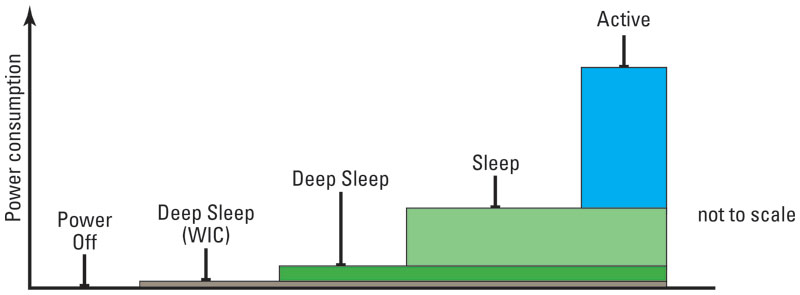
\includegraphics[width=\textwidth]{power-consumption}
  \caption{Енерговитрати процесора за різних профілів виконання}
\end{figure}

\subsection{GPIO (General-Purpose Input/Output)}

  Кількість виводів внутрішньої периферії процесора перевищує кількість наявних зовнішних виводів на корпусі. GPIO надає можливість назначити відповідність зовнішних виводів до внутрішніх. Окрім цього, GPIO надає можливість використати певні піни процесора як піни загального призначення, що можуть бути зконфігуровані як ввід або вивід (звідси назва). Ця можливість була використана для керування світлодіодами, що присутні на платі STM32F4Discovery.

\subsection{NVIC (Nested Vectored Interrupt Controller)}

Мікроконтроллери ARM приділяють значну увагу перериванням. Однією із особливостей серії Cortex-M є низькі затримки для обробки переривань. Контролер переривань підтримує до 240 переривань\cite{cortex-m:nvic}, кожен з яких може мати один із 256 рівнів пріоритету, що може змінюватися динамічно.

Контролер переривань і ядро процесора тісно пов'язані, що дозволяє зменшити затримку і ефективно оброблювати пізні переривання. Контролер переривань відслідковує вкладені переривання для реалізації хвостової обробки.

\begin{figure}[h]
  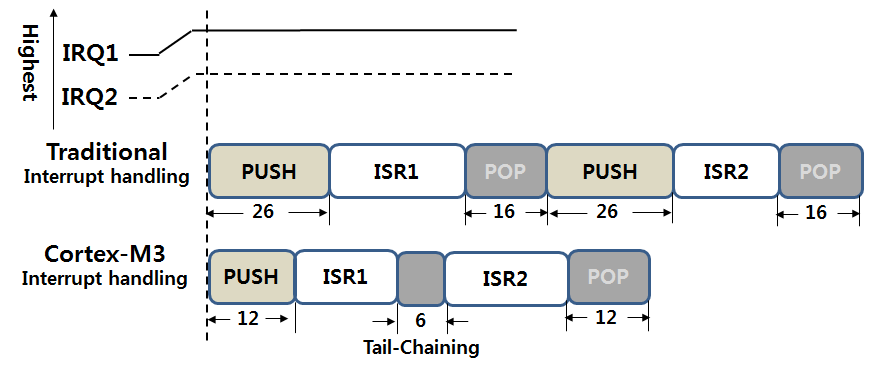
\includegraphics[width=\textwidth]{interrupt-tail-chaining}
  \caption{Приклад хвостової обробки переривань}\label{fig:interrupt-tail-chaining}
\end{figure}

Цікавим способом було реалізовано таблицю переривань. В середині модуля \code{stm32f4::isr\_vector} було оголошено назви всіх обробників переривань, що можуть існувати в системі, а також було сформовано масив з усіма обробника у тому порядку, що вимагає NVIC. Далі ця таблиця встановлюється у відповідне місце за допомогою лінкер-скрипту. Так само за допомогою лінкер скрипту було встановлено початкову адресу стеку (знаходиться безпосередньо перед таблицею переривань).

Це дозволило позбутися будь-якого асемблерного коду для ініціалізації ядра, і вся система наразі є повністю написана за допомогою мови Rust, що полегшує процес зборки.

\subsection{USART (Universal Synchronous\slash{}\hspace{0pt}Asynchronous Receiver\slash{}\hspace{0pt}Transmitter)}

  USART є відносно простим і розповсюдженим інтерфейсом передачі даних. Він був використаний для встановлення зв'язку із хост системою і надання можливості двустороннього обміну інформацією за допомогою консолі користувача і спеціального програмного забезпечення, що дозволяє працювати з RS-232. В якості такого програмного забезпечення було використано minicom.

  При підключені до пристрою, користувач має можливість бачити консоль пристрою і взаємодіяти з ним (надавати команди).

  Драйвер USART може працювати як в блокуючому (використовуючи активне очікування) так і неблокуючому (за допомогою переривань) режимах. Хоч блокуючий режим і йде проти ідеології даної системи управління, його зручно використовувати для відлагодження. Він використовується лише для обробки виключної ситуації в системі; для решти застосувань використовується неблокуючий режим.

\subsection{Таймери}

STM32F407VGT6 має набір різних внутрішніх таймерів. В рамках даного дипломного проекту було реалізовано драйвер для TIM2, TIM3, TIM4 і TIM5, що є таймерами загального призначення. Один із них було використано для тестування системи переривань; таймер TIM2 генерує періодичні переривання, і його обробник змінює стан діоду LD3 на протилежний.

\section{Термінал}

Система має простий емулятор терміналу, що доступний на USART1 на пінах PB6 (TX) і PB7 (RX) і використовує наступні параметри USART: baud-rate дорівнює 9600, 8-бітне слово, без перевірки парності, один стоп-біт.

Термінал має команди для друку вітання, виведення допомоги, включення і виключення будь-якого із чотирьох світлодіодів, що присутні на платі STM32F4Discovery, а також для введення системи в режим паніки (було використано для тестування виводу повідомлень про помилки).

\begin{figure}[!p]
  \fbox{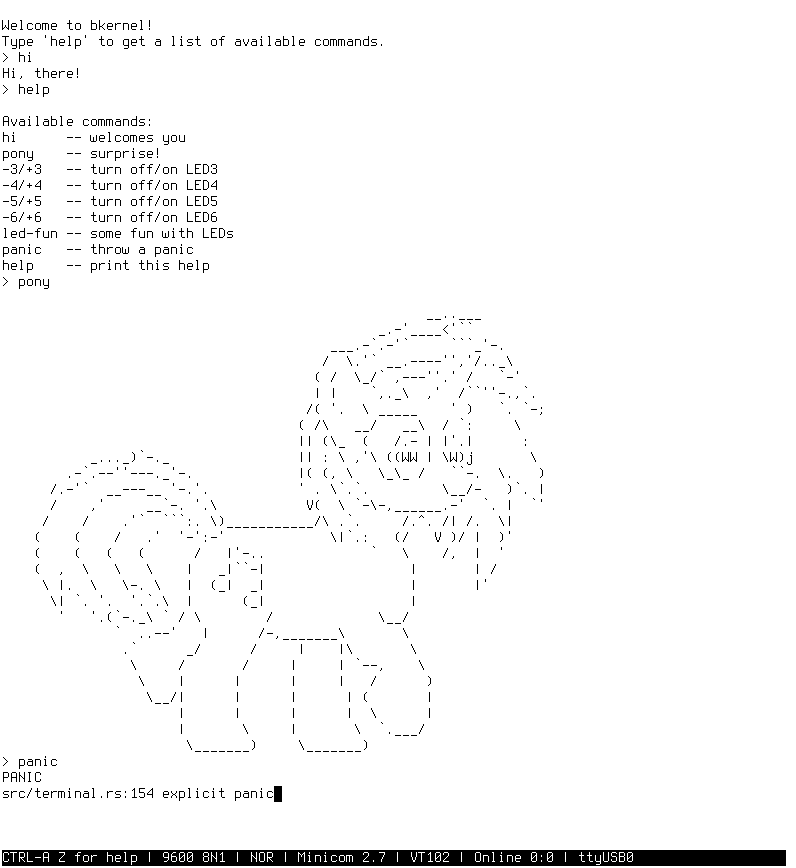
\includegraphics[width=\textwidth]{terminal}}
  \caption{Приклад роботи емулятора терміналу}\label{fig:terminal}
\end{figure}

Також, термінал підтримує просте редагування команд. На рисунку \ref{fig:terminal} зображено приклад роботи з емулятором терміналу.

\subsection{Rust}

Огляд мов програмування і обгрунтування вибору мови було виконано в розділі \ref{chap:languages}. В даному розділі опиане загальне враження від Rust у рамках побудови вбудованих операційних систем.

За весь час розробки Rust показав себе як з хорошого, так і поганого боків.

\begin{itemize}
\item Висока ефективність згеренованого машиного коду, а також виконання \ac{LTO}.

\item Велика кількість попереджень, що включені за замовчуванням. Це дозволяє підтримувати високу якість коду.

\item Включені за замовчуванням перевірки на вихід за границі масивів, а також цілочисельне переповнення дозволяють швидко знаходити і виправляти дані типи програмних помилок.

\item Ці перевірки неможливо виключити, що може негативно сказатися на швидкодії фінального продукту.

\item Сильна типізація дозволила знайти кілька програмних помилок на етапі компіляції. Однак, ручні конвертації між типами можуть бути надокучливими.

\item Недостатньо можливостей для роботи з константними виразами. Наразі ведеться активна розробка і вровадження константних функцій.

\item Для деяких типів неможливо мати глобальні змінні.

\item Відсутність голих функцій (функції без прологі і епілогу) заставляє обробників переривання виконувати зайву роботу. Вони зберігають стан в той час, як це було зроблено процесором при вході в обробник переривання.

\item Для написання низькорівневого коду доводиться використовувати нестабільний функціонал компілятора. Через це, з оновленням версії компілятора, код перестає збиратися. Ця проблема стає дуже гостро, оскільки буквально за кілька місяців код застаріває.

\item Деякі ідеї неможливо реалізувати через те, що вони порушують модель безпеки Rust. Це означає, що необхідно реалізовувати менш ефективні, або більш складні варіанти, ніж було заплановано початково.
\end{itemize}

В цілому, враження від мови Rust є позитивним. Мова активно розвивається і додає все більше можливостей, що необхідні при низькорівневому програмуванні.

Однак, насьогодні Rust ще не готовий для програмування промислових вбудованих систем.

\chapterconslusions{}

В даному розділі було описано процес і результат реалізації системи.

При розробці було використано найсучасніші технології і інструменти, що дозволяють значно пришвидшити розробку програмних продуктів, зменшуючи навантаження на програміста і ймовірність програмної помилки.

Релізована система займає 188 байт оперативної пам'яті, не враховуючи програмний стек. Максимальний зафіксований об'єм стеку дорівнює 76 байтам. Загальний об'єм використаної пам'яті дорівнює 264 байтам.

\specialchapter{Висновки}

Даний дипломний проект присвячений розгляду проблеми реалізації систем управління для вбудованих систем, а також вбудованих систем реального часу. Метою роботи було створення операційної системи для вирішення цієї проблеми.

Було розглянуто теоретичну базу даної предметної області, а також детально розібрано вже готові реалізації подібних систем. З даного дослідження були встановлені вимоги до системи і її основний функціонал. Було проведено аналіз доступних мов програмування і інструментів, та обрано мову Rust для реалізації.

Реалізована система потребує дуже малий об'єм оперативної пам'яті, а також є досить зручною у використанні.

\begin{thebibliography}{00}
  \bibitem{linux}
    \eresource{Linux.com | The source for Linux information}{https://linux.com/}
  \bibitem{linux-galileo}
    \eresource{microYocto and the Internet of Tiny}{http://events.linuxfoundation.org/sites/events/files/slides/tom.zanussi-elc2014.pdf}
  \bibitem{intel-galileo}
    \eresource{Galileo Feature Sheet}{http://www.intel.com/content/dam/support/us/en/documents/galileo/sb/galileo\_datasheet\_329681\_003.pdf}

  \bibitem{freertos}
    \eresource{FreeRTOS - Market leading RTOS (Real Time Operating System) for embedded systems with Internet of Things extensions}{http://www.freertos.org/}
  \bibitem{freertos:popular}
    \eresource{Android, FreeRTOS top EE Times' 2013 embedded survey}{http://www.eetimes.com/document.asp?doc\_id=1263083}
  \bibitem{freertos:license}
    \eresource{FreeRTOS License}{http://www.freertos.org/license.txt}
  \bibitem{openrtos}
    \eresource{OPENRTOS, part of embedded FreeRTOS -- OpenRTOS -- SafeRTOS family}{http://www.highintegritysystems.com/openrtos/}

  \bibitem{vxworks}
    \eresource{VxWorks}{http://windriver.com/products/vxworks/}
  \bibitem{vxworks:rovers}
    \eresource{Inside NASA's Curiosity: It's an Apple Airport Extreme... with wheels | ExtremeTech}{http://www.extremetech.com/extreme/134041-inside-nasas-curiosity-its-an-apple-airport-extreme-with-wheels}
  \bibitem{vxworks:boeing}
    \eresource{787 Dreamliner (Common Core Systems) | Customers | AdaCore}{http://www.adacore.com/customers/787-dreamliner-common-core-system/}

  \bibitem{qnx}
    \eresource{QNX Neutrino RTOS}{http://www.qnx.com/products/neutrino-rtos/neutrino-rtos.html}
  \bibitem{qnx:noncommercial}
    \eresource{QNX Neutrino Realtime Operating System}{http://www.qnx.com/download/download.html?dlc=proc&newsearch=yes&searchme=non-commercial&p=1&sort=bydate&sorttype=desc&searchdate=alltime}

  \bibitem{dave-evans:IoT}
    \eresource{The Internet of Things. How the Next Evolution of the Internet is Changing Everything}{http://www.cisco.com/c/dam/en\_us/about/ac79/docs/innov/IoT\_IBSG\_0411FINAL.pdf}
  \bibitem{stewart-bill:history-of-c}
    \eresource{History of C Programming Language}{http://www.livinginternet.com/i/iw\_unix\_c.htm}

  \bibitem{idris}
    \eresource{Idris | A Language with Dependent Types}{http://www.idris-lang.org/}
  \bibitem{idris:first-release}
    \eresource{idris: Dependently Typed Functional Programming Language}{http://hackage.haskell.org/package/idris-0.1.3}
  \bibitem{haskell:atom}
    \eresource{atom: An EDSL for embedded hard realtime applications}{https://hackage.haskell.org/package/atom}
  \bibitem{haskell:ivory}
    \eresource{Ivory - index}{http://ivorylang.org/index.html}
  \bibitem{haskell}
    \eresource{Haskell Language}{https://www.haskell.org/}

  \bibitem{nim}
    \eresource{Nim Programming Language}{http://nim-lang.org/}
  \bibitem{nim:directives}
    \eresource{Nim Manual}{http://nim-lang.org/docs/manual.html\#pragmas}
  \bibitem{nim:volatile}
    \eresource{\{.volatile.\} is almost useless · Issue \# 3382 · nim-lang/Nim}{https://github.com/nim-lang/Nim/issues/3382}

  \bibitem{rust}
    \eresource{The Rust Programming Language}{https://www.rust-lang.org/}
  \bibitem{rust:mozilla}
    \eresource{The Rust Language | Lambda the Ultimate}{http://lambda-the-ultimate.org/node/4009}
  \bibitem{llvm}
    \eresource{The LLVM Compiler Infrastructure Project}{http://llvm.org/}

  \bibitem{nix}
    \eresource{Nix: The Purely Functional Package Manager}{http://nixos.org/nix/}
  \bibitem{gnu-make}
    \eresource{Make - GNU Project - Free Software Foundation}{https://www.gnu.org/software/make/}
  \bibitem{cargo}
    \eresource{Cargo}{https://crates.io/}
  \bibitem{gcc-arm-embedded}
    \eresource{GCC ARM Embedded in Launchpad}{https://launchpad.net/gcc-arm-embedded}
  \bibitem{openocd}
    \eresource{Open On-Chip Debugger}{http://openocd.org/}
  \bibitem{expect}
    \eresource{Expect - Expect - Home Page}{http://expect.sourceforge.net/}
  \bibitem{tcl}
    \eresource{Tcl Developer Site}{https://www.tcl.tk/}
  \bibitem{minicom}
    \eresource{Alioth: minicom: Project Home}{https://alioth.debian.org/projects/minicom}

  \bibitem{cortex-m:nvic}
    \eresource{ARM Information Center}{http://infocenter.arm.com/help/index.jsp?topic=/com.arm.doc.ddi0337e/Cihcffda.html}

  \bibitem{embedded:99}
    \eresource{Real men program in C | Embedded}{http://www.embedded.com/electronics-blogs/barr-code/4027479/Real-men-program-in-C}
  \bibitem{linux:schedulers}
    \eresource{Real-Time Linux Kernel Scheduler | Linux Journal}{http://www.linuxjournal.com/magazine/real-time-linux-kernel-scheduler}

  \bibitem{synthesis}
    Massalin H. Synthesis: An Efficient Implementation of Fundamental Operating System Services. -- Columbia University, 1992. -- 158 c.

\end{thebibliography}

% \appendix
% \chapter{}

\finalizepart{}

\end{document}
